
\begin{figure}
\center


\begin{comment}
python3 CounterfactualModel_VIZ_Components.py 2 0 10.0 180 1000 STEEPSHIFTED STEEPPERIODIC 5        
\end{comment}

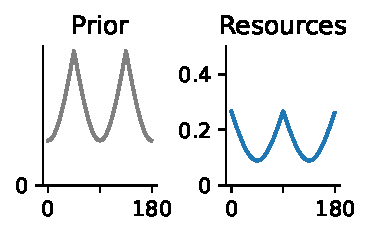
\includegraphics[width=0.35\textwidth]{figures/CounterfactualModel_VIZ_Components.py_5_STEEPSHIFTED_STEEPPERIODIC_2_0_10.0_180.pdf}
%%%%%%%

  \begin{tabular}{@{}c@{}c@{}c@{}}
    % Row 1
    $p=0$ & $p=1$ & $p=2$ \\[-1.4ex]
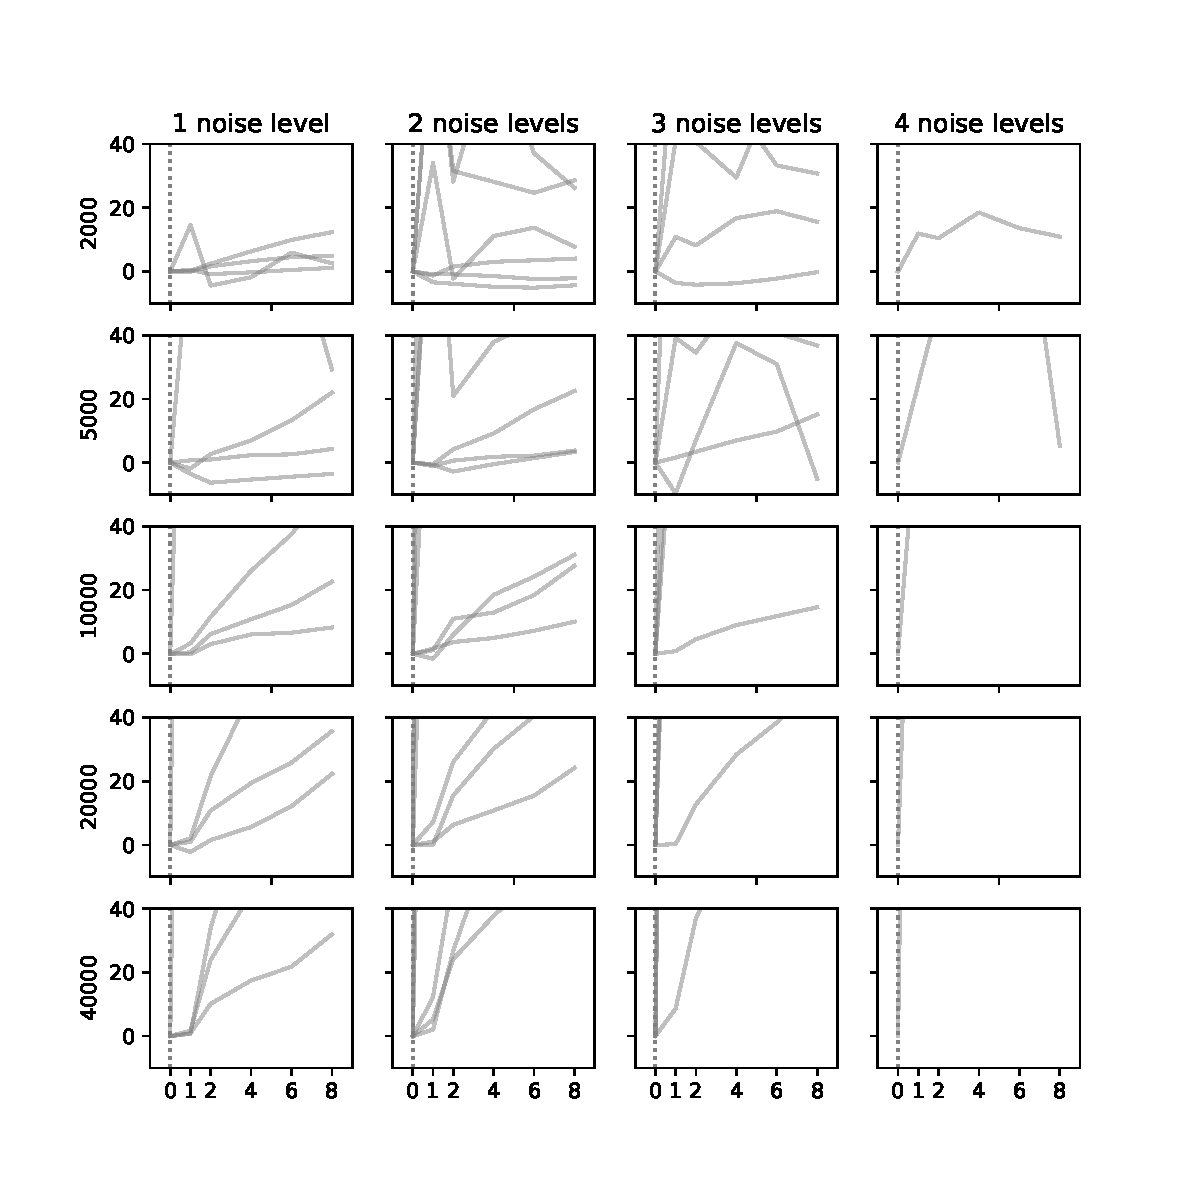
\includegraphics[width=0.33\textwidth]{figures/evaluateCrossValidationResults_Synthetic_Gardelle_VisualizeByNoiseCount_AndSize_ByP_Poster_Exculde1.py_STEEPSHIFTED_STEEPPERIODIC_0.pdf} &
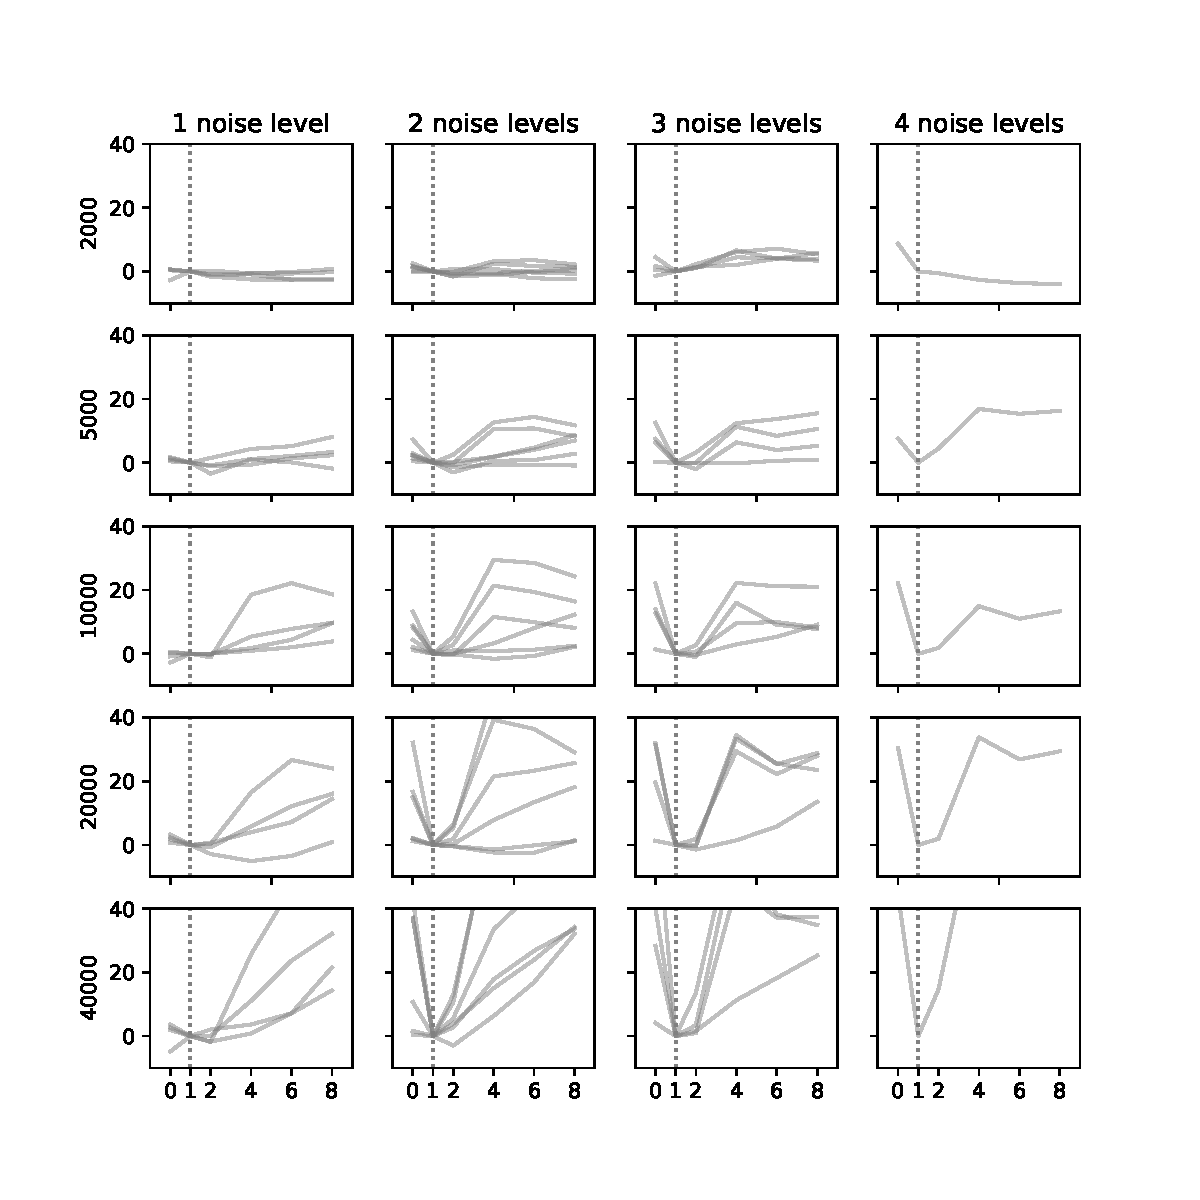
\includegraphics[width=0.33\textwidth]{figures/evaluateCrossValidationResults_Synthetic_Gardelle_VisualizeByNoiseCount_AndSize_ByP_Poster_Exculde1.py_STEEPSHIFTED_STEEPPERIODIC_1.pdf} &
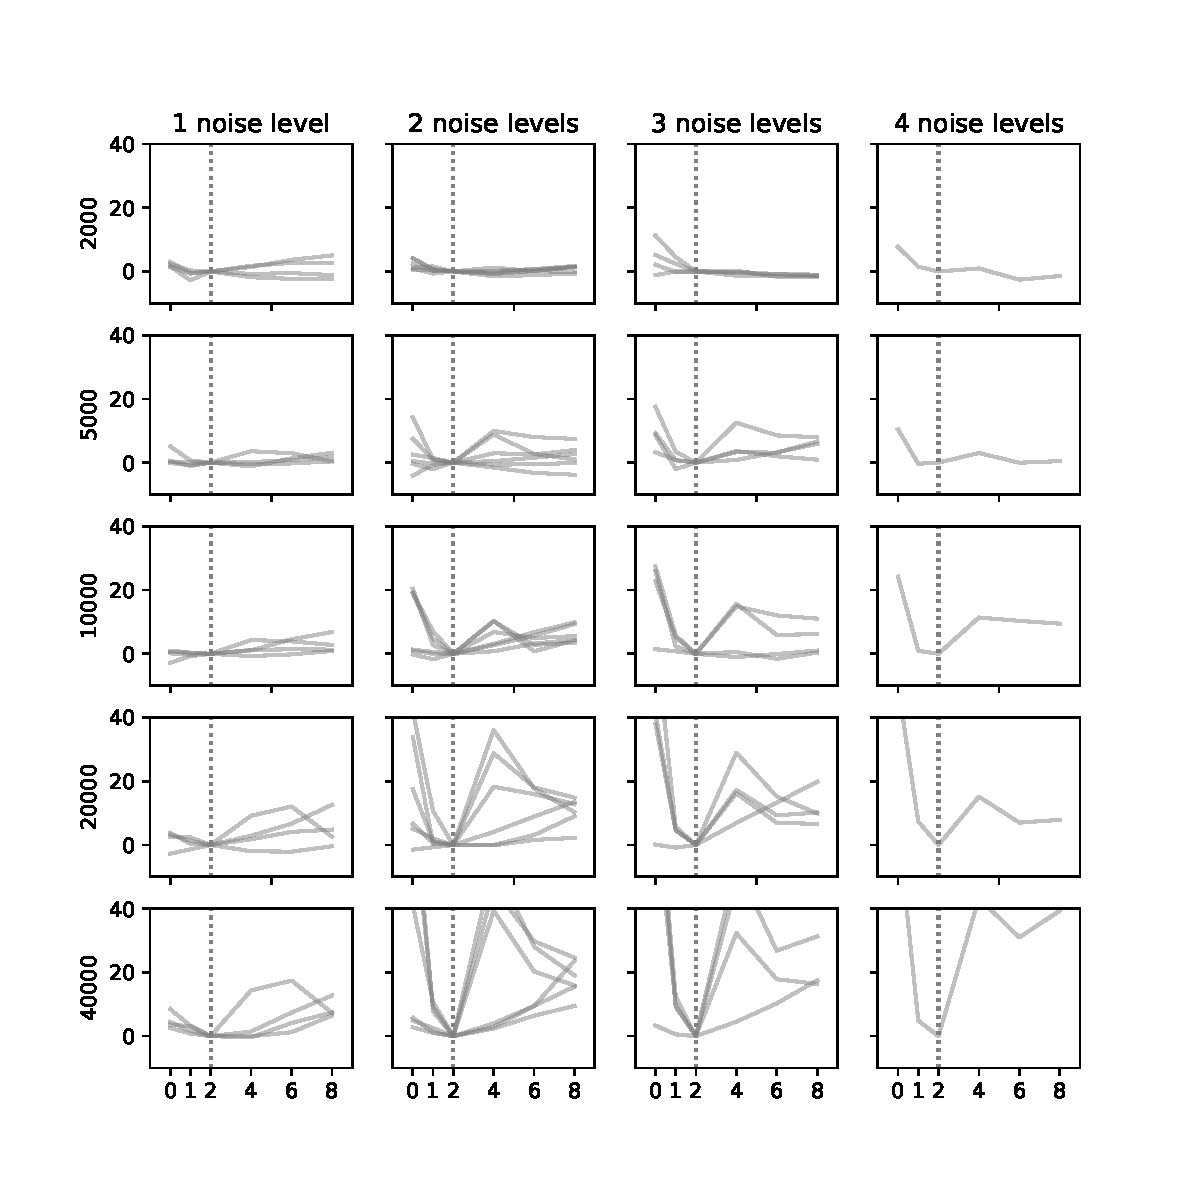
\includegraphics[width=0.33\textwidth]{figures/evaluateCrossValidationResults_Synthetic_Gardelle_VisualizeByNoiseCount_AndSize_ByP_Poster_Exculde1.py_STEEPSHIFTED_STEEPPERIODIC_2.pdf} \\[-2ex]
$p=4$ &    $p=6$ & $p=8$ \\[-1.4ex]
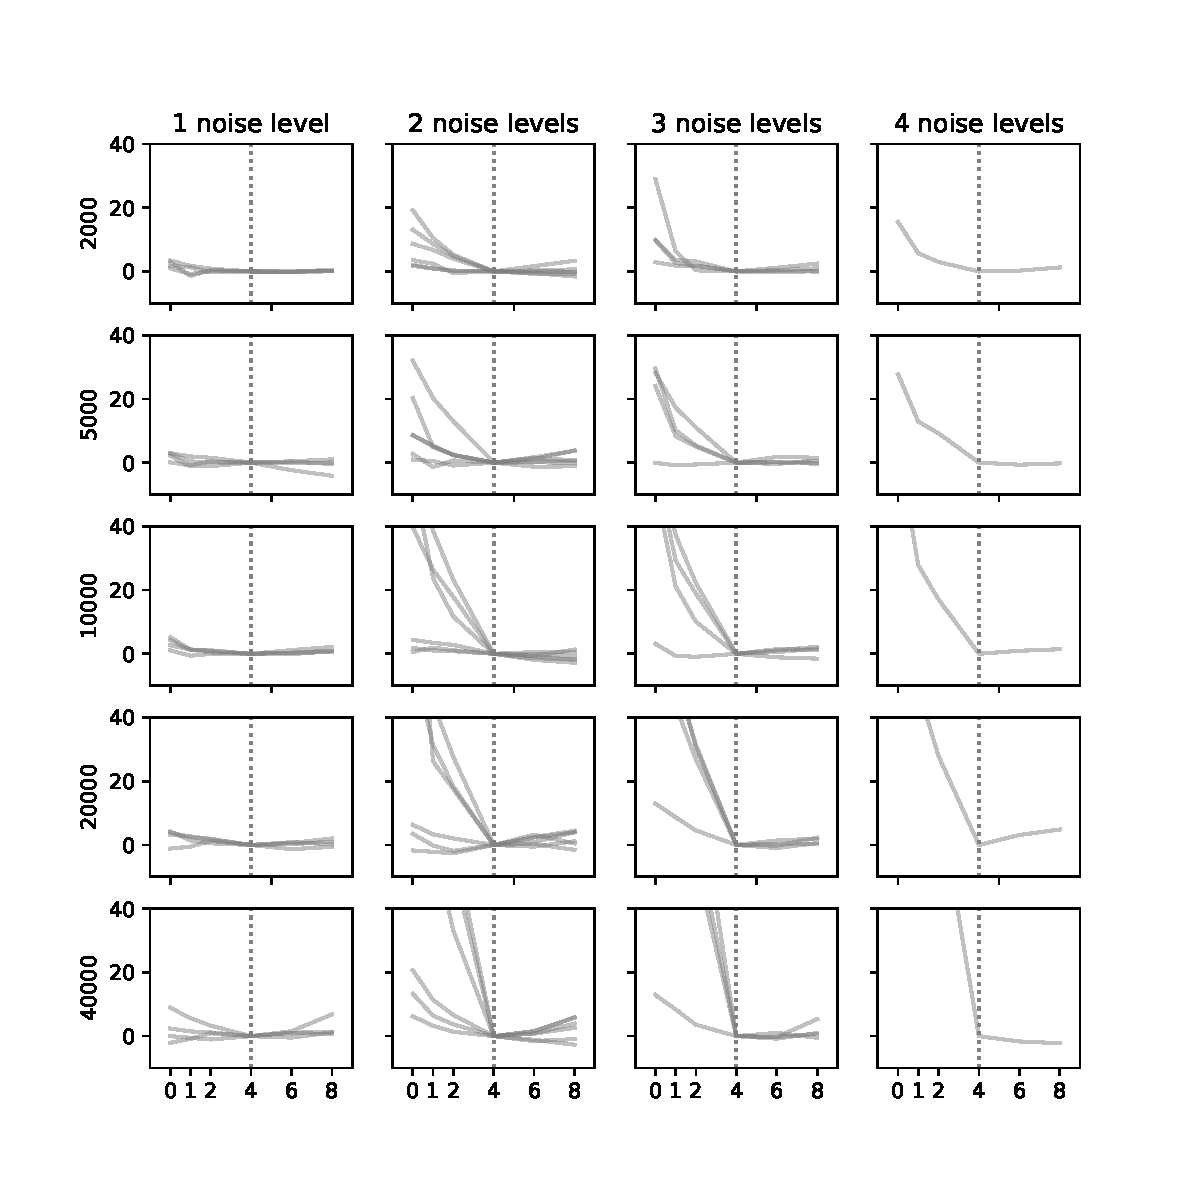
\includegraphics[width=0.33\textwidth]{figures/evaluateCrossValidationResults_Synthetic_Gardelle_VisualizeByNoiseCount_AndSize_ByP_Poster_Exculde1.py_STEEPSHIFTED_STEEPPERIODIC_4.pdf} &
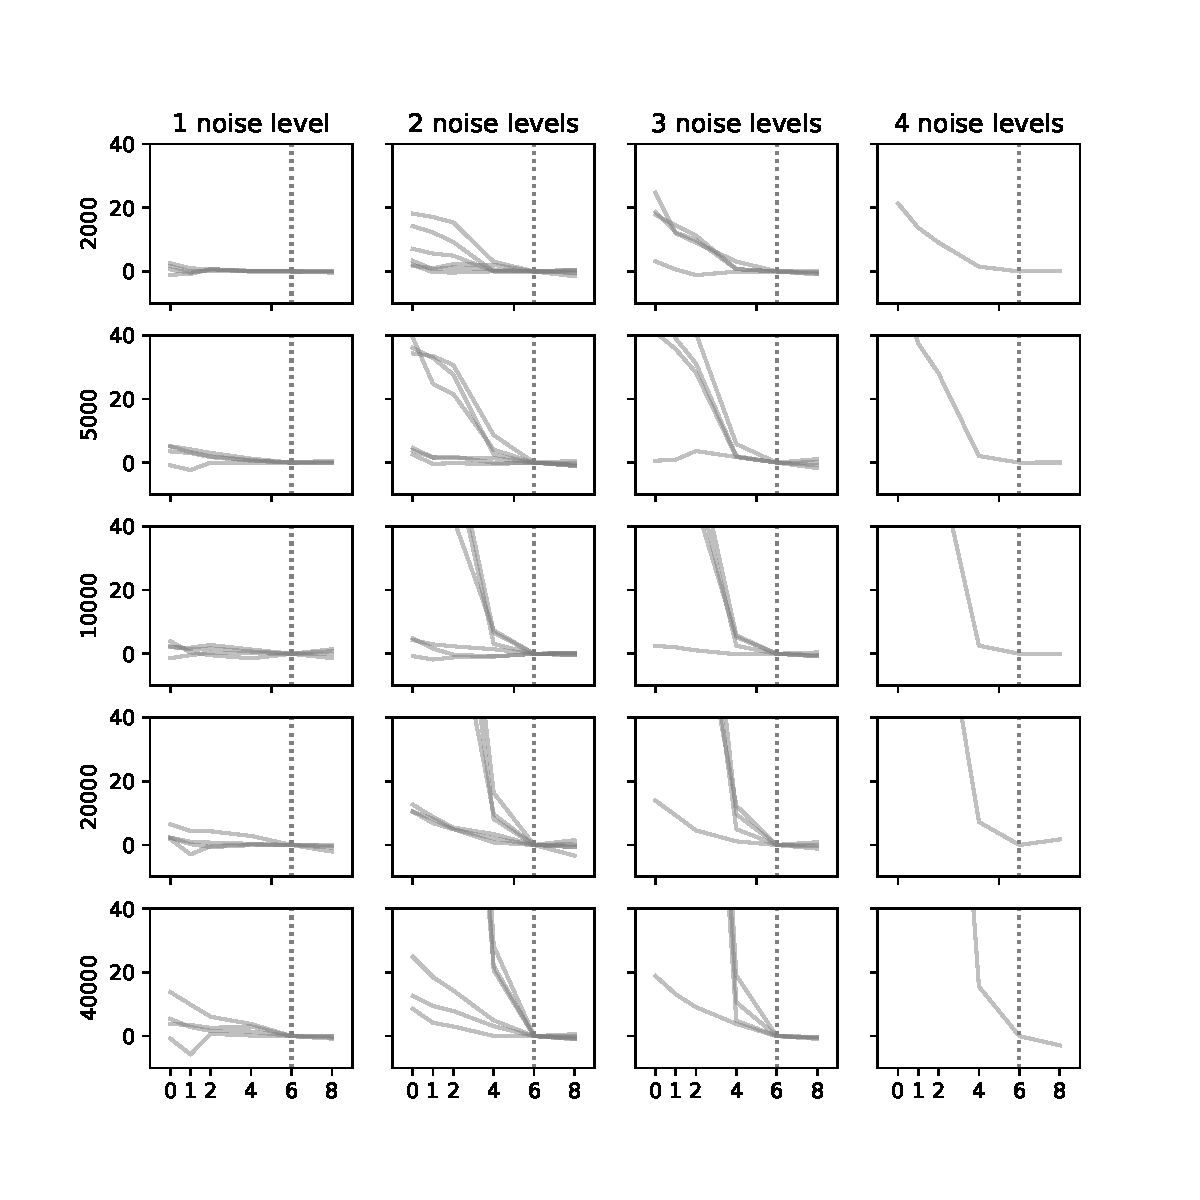
\includegraphics[width=0.33\textwidth]{figures/evaluateCrossValidationResults_Synthetic_Gardelle_VisualizeByNoiseCount_AndSize_ByP_Poster_Exculde1.py_STEEPSHIFTED_STEEPPERIODIC_6.pdf} &
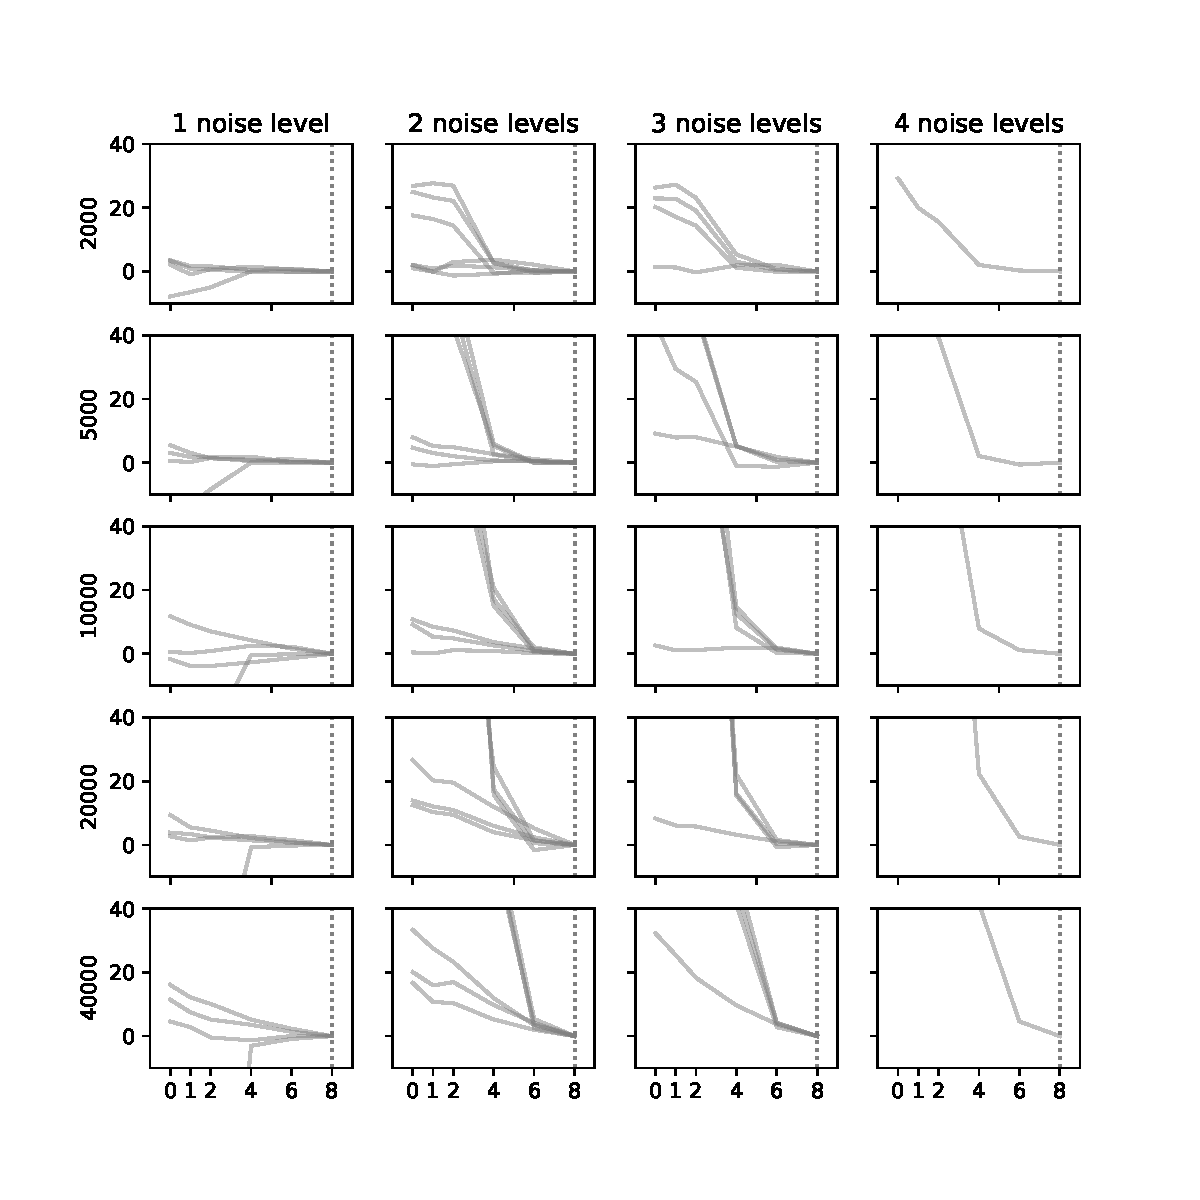
\includegraphics[width=0.33\textwidth]{figures/evaluateCrossValidationResults_Synthetic_Gardelle_VisualizeByNoiseCount_AndSize_ByP_Poster_Exculde1.py_STEEPSHIFTED_STEEPPERIODIC_8.pdf}
  \end{tabular}
\vspace{-4mm}
\caption{Circular Stimulus Space:
Identifiability of the loss function depending on the number of trials (rows, from 2K to 40K), the number of of sensory noise levels (columns, from 1 to 4), and the ground truth loss function exponent (facets, $p$ from 0 to 8).
Each curve represents one synthetic dataset with the given number of trials and noise levels, with the prior and encoding resources shown at the top.
In each case, we include all possible combinations of the four overall noise levels, i.e., there are four cases at 1 noise level, ${4 \choose 2} = 6$ combinations at 2 noise levels, ${4 \choose 3} = 4$ combinations at 3 noise levels, and a single combination at 4 noise levels.
We plot the model fit at each exponent as quantified by the difference to model fit at the ground-truth exponent, whose position is indicated with a dotted vertical line.
Note that, in order to keep the y-axis range consistent across panels for easy comparison, values greater than 40 are not shown.
}
\label{fig:recover-loss-circ-shifted-periodic}

\end{figure}


